\documentclass[]{article}

% Imported Packages
%------------------------------------------------------------------------------
\usepackage{amssymb}
\usepackage{amstext}
\usepackage{amsthm}
\usepackage{amsmath}
\usepackage{enumerate}
\usepackage{fancyhdr}
\usepackage[margin=1in]{geometry}
\usepackage{graphicx}
\usepackage{extarrows}
\usepackage{setspace}
%------------------------------------------------------------------------------

% Header and Footer
%------------------------------------------------------------------------------
\pagestyle{plain}  
\renewcommand\headrulewidth{0.4pt}                                      
\renewcommand\footrulewidth{0.4pt}                                    
%------------------------------------------------------------------------------

% Title Details
%------------------------------------------------------------------------------
\title{Deliverable \#3 Template}
\author{SE 3A04: Software Design II -- Large System Design}
\date{}                               
%------------------------------------------------------------------------------

% Document
%------------------------------------------------------------------------------
\begin{document}

\maketitle	

\section{Introduction}
\label{sec:introduction}
% Begin Section

%This section should provide an brief overview of the entire document.

\subsection{Purpose}
\label{sub:purpose}
% Begin SubSection
%\begin{enumerate}[a)]
%	\item Delineate the purpose of the document
%	\item Specify the intended audience for the document
%\end{enumerate}
% End SubSection
The purpose of this document is to give a greater description of the application NatureOptix. This is to be done by providing diagrams and charts. The charts and diagrams to be given are state diagrams for each controller class, sequence diagrams for each business event, and a detailed class diagram. It is the intent of this document to give the audience a more detailed look of the overall system of NatureOptix. 
\subsection{System Description}
\label{sub:system_description} 
% Begin SubSection
%\begin{enumerate}[a)]
%	\item Give a brief description of the system. This could be a paragraph or two to give some context to this document.
%\end{enumerate}
The NatureOptix application will allow the user to identify a natural phenomena. The application will ask the user a series of questions and the user will be able to specify an answer for each question from a drop down menu. The application will use a combination of Repository and Blackboard Architecture. It will be comprised of 9 entities; 3 experts ( a physicist, a field expert, and a meteorologist), a location expert, a database corresponding to attributes identified by each one of the experts for every optical natural phenomena, and a controller. Each database will contain information about each phenomena specific to what it's expert knows. Each expert will act as an algorithm that compares characteristics of a phenomena in the database to the user input. The physicist will compare the visual attributes, the field expert will compare the physical attributes, and the meteorologist will compare the weather condition attributes required for each phenomena to occur. Each expert will create a list of phenomena that has characteristics that match the user input. The three lists will then be sent to the controller. The controller will determine what phenomenon is common to all three lists and will present this phenomenon to the user. In some boundary cases, the applications shall provide the users with an aggregated list of closest match results to their query. The experts will not be able to communicate to each other and will only be communicating with the database and controller. 
% End SubSection

\subsection{Overview}
\label{sub:overview}
% Begin SubSection
%\begin{enumerate}[a)]
%	\item Describe what the rest of the document contains 
%	\item Explain how the document is organised
%\end{enumerate}
The remainder of the document is separated into three sections. These sections are State Charts for the Controller Classes, Sequence Diagrams, and Detailed Class Diagrams. Each section does not have subsections.
% End SubSection

% End Section

\section{State Charts for Controller Classes}
\label{sec:state_charts_for_controller_classes}
% Begin Section
This section should provide a state chart for each controller class for your application.
% End Section
 
\section{Sequence Diagrams}
\label{sec:sequence_diagrams}
% Begin Section
****help insert images!!!!*****
\begin{figure}[!hb]
	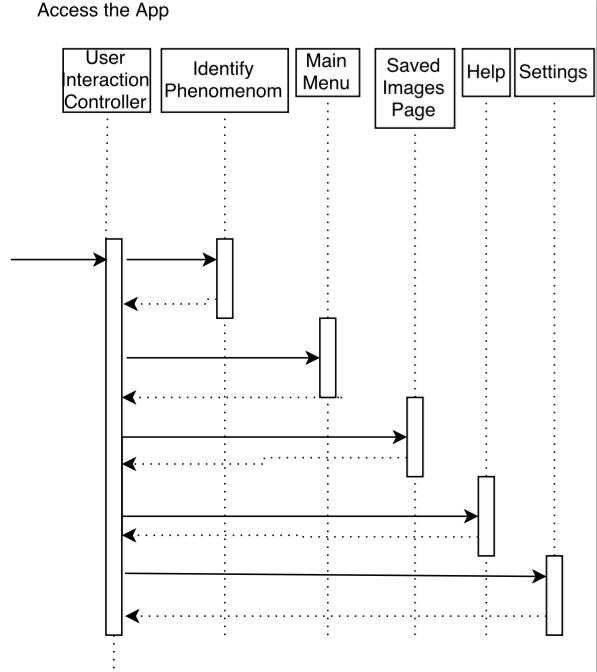
\includegraphics[width=\linewidth]{sequenceDiagram1.png}
	\caption{Sequence Diagram for Accessing the Application}
\end{figure}
\begin{figure}[!hb]
	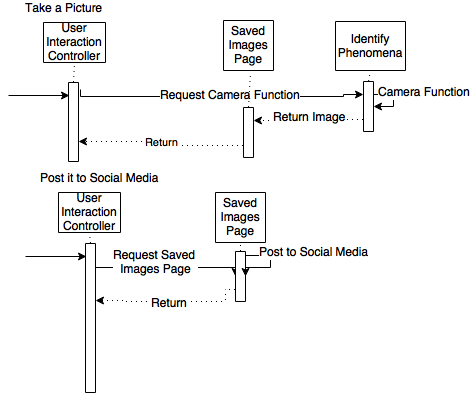
\includegraphics[width=\linewidth]{sequenceDiagram2.png}
	\caption{Sequence Diagram for Taking a Picture and Posting it to Social Media}
\end{figure}
\begin{figure}[!hb]
	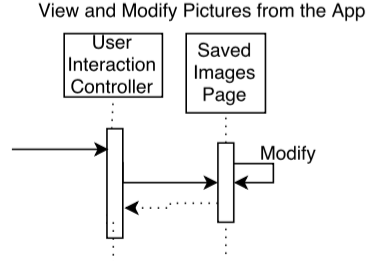
\includegraphics[width=\linewidth]{sequenceDiagram3.png}
	\caption{Sequence Diagram for Viewing and Modifying Pictures from the Application}
\end{figure}
\begin{figure}[!hb]
	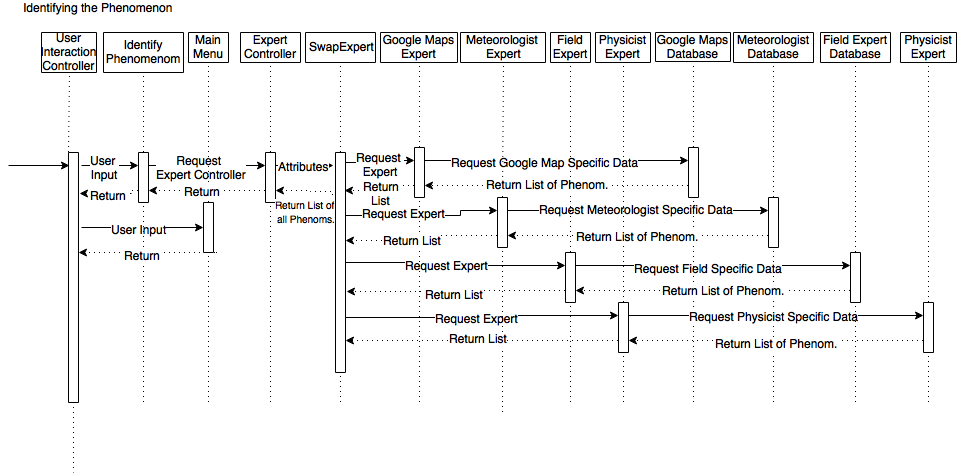
\includegraphics[width=\linewidth]{sequenceDiagram4.png}
	\caption{Sequence Diagram for Identifying the Phenomenon}
\end{figure}

% End Section

\section{Detailed Class Diagram}
\label{sec:detailed_class_diagram}
% Begin Section
This section should provide a detailed class diagram for your application.
% End Section

\appendix
\section{Division of Labour}
\label{sec:division_of_labour}
% Begin Section
Include a Division of Labour sheet which indicates the contributions of each team member. This sheet must be signed by all team members.
% End Section

\newpage
\section*{IMPORTANT NOTES}
\begin{itemize}
	\item You do \underline{NOT} need to provide a text explanation of each diagram; the diagram should speak for itself
	\item Please document any non-standard notations that you may have used
	\begin{itemize}
		\item \emph{Rule of Thumb}: if you feel there is any doubt surrounding the meaning of your notations, document them
	\end{itemize}
	\item Some diagrams may be difficult to fit into one page
	\begin{itemize}
		\item It is OK if the text is small but please ensure that it is readable when printed
		\item If you need to break a diagram onto multiple pages, please adopt a system of doing so and throughly explain how it can be reconnected from one page to the next; if you are unsure about this, please ask me
	\end{itemize}
	\item Please submit the latest version of Deliverable 1 and Deliverable 2 with Deliverable 3
	\begin{itemize}
		\item They do not have to be a freshly printed versions; the latest marked versions are OK
	\end{itemize}
	\item If you do \underline{NOT} have a Division of Labour sheet, your deliverable will \underline{NOT} be marked
\end{itemize}


\end{document}
%------------------------------------------------------------------------------